\section{Software Design Document}

	\subsection{Introduction}
		\subsubsection{Purpose}
			This document is written, to document the proposed architecture of a research environment for the optimal layout of graph records on disk. The document is inteded for the developers implementing the system, the persons supervising projects using the final system and the other stakeholders to get an overview of the software system.
			
		\subsubsection{Scope}
			This Software system shall implement a graph record layout research environment, that consists of a graph database along with tools, that rearranges the recrods of the database based on a predefined format, measure the number of disk accesses needed to service a certain query and that provide other layouts to compare against.
		
		
        \subsubsection{Definitions, Acronyms, Abbreviations}
        \begin{longtable}{|>{\raggedright \arraybackslash}p{0.35\textwidth}||
        >{\raggedright \arraybackslash}p{0.15\textwidth}|>{\raggedright \arraybackslash}p{0.5\textwidth}|} \hline

        word & shortform & meaning \\ \hline
        database & db & a software system to store and alter data in an organized manner. \\ \hline
        Operating System & os & An operating system is system software that manages computer hardware, software resources, and provides common services for computer programs. \\ \hline
        Portable Operating System Interface & POSIX & A specification for a set of OSes that covers for example Linux, macOS and BSD-style operating systems. \\ \hline
        C Programming Language & C & a programming language. \\ \hline
        Input/Output & IO & the notion of loading and storing information to media other than RAM and CPU registers. In this document hard drive and solid state disk are meant primarily. \\ \hline
        Create, read, update, delete & CRUD & The basic database operations, that allow to create, read, update and delete a record. \\ \hline
        Databases and Information Systems & DBIS & The name of the group at the university of Konstanz, at which the software system is build. \\ \hline
        Stanford Network Analytics Project & SNAP & A porject of the university of stanford that hosts many large scale graph data sets.  \\ \hline
        Least Recently Used & LRU & A strategy when evicting pages from a pool of memory. \\ \hline
        Breadth-first Search & BFS & A graph traversal scheme, where all neighbours of the current node are visited before continuing with the next node. \\ \hline
        Depth-first Search & DFS & A graph traversal scheme, where the next node is considered before visiting all neighbours of the current node. \\ \hline
        Single Source Shortest Path & SSSP & The problem of finding the shortest path to all nodes in a graph from one source node. \\ \hline
        \dots & \dots & \dots \\ \hline
        \hline
        \end{longtable}
	
		\subsubsection{References}
			\begin{enumerate}
				\item SRS Document
				\item Neo4J record structure documentation
			\end{enumerate}
			
		\subsubsection{Overview}
			The proposed architecture will be shown from a static point of view, e.g. the decomposition into subsystems and their structure. Then the dynamic aspects of the system are following. This contains the description of interfaces between components, the behavior of the system and information flow. Finally, used design patterns are mentioned.
			
			
	\subsection{Software Architecture}
		\subsubsection{Overview}
		The graph record layout research environment consists of a database and a set of functions to assist in reordering records, measuring the number of IOs of a certain layout, visualizing the results, queries with certain access patterns, and an interface to implement new layout methods easily into the environment.
			\begin{description}
				\item [IO] 
				\item [Cache]
				\item [Access] 
				\item [Queries] 
				\item [Import] 
				\item [Layout Utilities] 
				\item [Layout Methods] 
				\item [Visualization Utilities]
			\end{description}
			
		\subsubsection{Subsystem decomposition}

			\paragraph{IO}
				The storage module shall provide IO methods, the concepts of a file, a page and a disk manager to manage and keep references to the afore mentioned. \\
                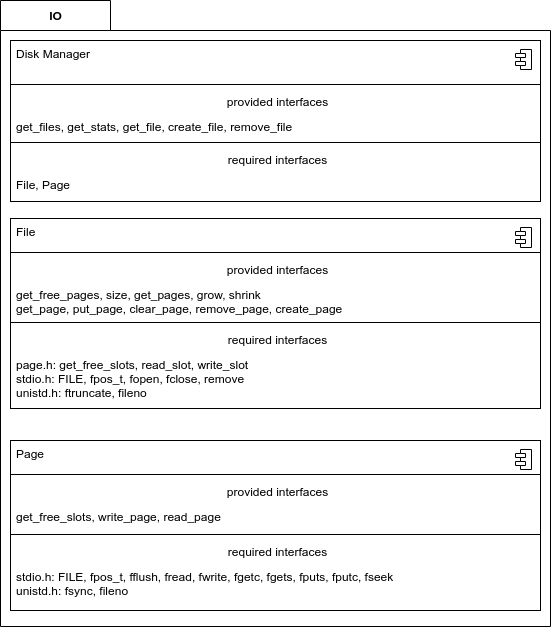
\includegraphics[keepaspectratio, width=\textwidth]{img/io_arch.png} \\

			\paragraph{Cache}
				This module shall provide the simplest for of a n page cache.
				Further it shall provide a basic one page buffer manager, i.e. implement the notions of a frame and the cache/buffer manager itself.   \\
                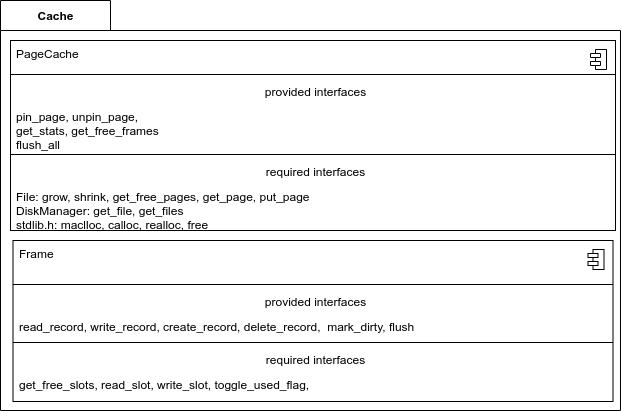
\includegraphics[keepaspectratio, width=\textwidth]{img/cache_arch.png} \\

            
            \paragraph{Record Structures}
            Finally the layout of the records and the structs to keep them in memory shall be described. Read and write operations shall be specified by these structs and contained as function pointers. The records must follow the index free adjacency list schema used in Neo4J.  
            This directory contains the structs and read/write functions of nodes and relationships \\
            
            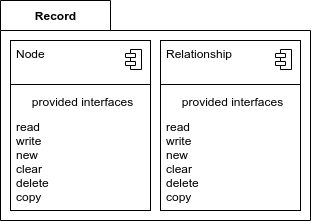
\includegraphics[keepaspectratio, width=\textwidth]{img/record_arch.png} \\

			
			\paragraph{Access}
				This module shall provide access operators for the database. That is it shall provide the following operators:
				\begin{itemize}
				 \item createNode
				 \item createRelationship
				 \item getNode
				 \item getRelationship
				 \item get Nodes
				 \item getRelationships
				 \item getNodesInRange
				 \item getRelationshipsInRange
				 \item Expand
				 \item filter
				\end{itemize}
                
                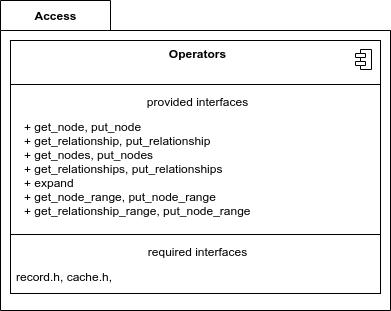
\includegraphics[keepaspectratio, width=\textwidth]{img/access_arch.png} \\


			
			\paragraph{Queries}
                Further is shall provides functions that use the other modules in order to generate access patterns, that is sequences of records and thus also disk blocks retreived from disk.
                The first query to be considered is breadth first search. Additionally Dijkstras algorithm and the A* algorithm are planned to be considered. Another class of possible queries to consider are random walks.

				
			\paragraph{Import}
				
			\paragraph{Layout Utilities}
			
			\paragraph{Visualization Utilities}
			
			\paragraph{Layout Method Interface}
			\begin{verbatim}
Interface MessagingService {
  public void sendMessage(string sender,
      string accesstoken, string recipient, Message message) {
    require accessValid(username, accessToken);
    require messageHandle != null;
    require message.length > 0;
    ensure getMessages(recipient, database.getUser(recipient)
        .getAccessToken()).contains(message);
  }

  public Message[] messages getMessages(string username, string accessToken) {
    require accessValid(username, accessToken);
    require messageHandle != null;
    ensure messages != null;
  }

  public void messageRead(String username, string accessToken Message message) {
    require accessValid(username, accessToken);
    require message != null;
    require getMessages(username, accessToken).contains(message);
    ensure !getMessages(username, accessToken).contains(message);
  }
}
\end{verbatim}
				
        

